% ============================================================
% appendix_draft.tex
% Copy contents into Chapters/appendix.tex
% ============================================================


\section*{Appendix}
\addcontentsline{toc}{section}{Appendix}

\appendix
\renewcommand{\thesection}{\Alph{section}}
\setcounter{section}{0}

\section{Euro Stoxx 50 Sample Constituents}
\label{app:tickers}

Table~\ref{tab:tickers} lists all 50 stocks included in the study. Tickers follow the Yahoo Finance convention and encode the primary exchange through their suffix: \texttt{.AS} = Euronext Amsterdam, \texttt{.PA} = Euronext Paris, \texttt{.DE} = Xetra Frankfurt, \texttt{.MC} = Bolsa de Madrid, \texttt{.MI} = Borsa Italiana, \texttt{.BR} = Euronext Brussels, \texttt{.HE} = Nasdaq Helsinki, \texttt{.L} = London Stock Exchange. All stocks were constituents of the Euro Stoxx 50 index at the time of data collection. Daily adjusted OHLCV data cover 1 January 2000 through 1 May 2026.

\begin{table}[H]
\centering
\caption{Euro Stoxx 50 Constituents Used in the Study}
\label{tab:tickers}
\resizebox{\textwidth}{!}{%
\begin{tabular}{rll@{\hspace{0.8cm}}rll}
\toprule
\textbf{No.} & \textbf{Ticker} & \textbf{Company}
& \textbf{No.} & \textbf{Ticker} & \textbf{Company} \\
\midrule
 1  & ABI.BR    & Anheuser-Busch InBev    & 26 & IFX.DE    & Infineon Technologies  \\
 2  & AD.AS     & Ahold Delhaize          & 27 & INGA.AS   & ING Group              \\
 3  & ADS.DE    & Adidas                  & 28 & ISP.MI    & Intesa Sanpaolo        \\
 4  & ADYEN.AS  & Adyen                   & 29 & ITX.MC    & Inditex                \\
 5  & AI.PA     & Air Liquide             & 30 & KER.PA    & Kering                 \\
 6  & AIR.PA    & Airbus                  & 31 & MBG.DE    & Mercedes-Benz Group    \\
 7  & ALV.DE    & Allianz                 & 32 & MC.PA     & LVMH                   \\
 8  & ASML.AS   & ASML Holding            & 33 & MUV2.DE   & Munich Re              \\
 9  & BAS.DE    & BASF                    & 34 & NDA-FI.HE & Nordea Bank            \\
10  & BAYN.DE   & Bayer                   & 35 & NOKIA.HE  & Nokia                  \\
11  & BBVA.MC   & BBVA                    & 36 & OR.PA     & L'Or\'{e}al            \\
12  & BMW.DE    & BMW Group               & 37 & PRX.AS    & Prosus                 \\
13  & BN.PA     & Danone                  & 38 & RI.PA     & Pernod Ricard          \\
14  & BNP.PA    & BNP Paribas             & 39 & RMS.PA    & Herm\`{e}s International \\
15  & CRH.L     & CRH                     & 40 & SAF.PA    & Safran                 \\
16  & CS.PA     & AXA                     & 41 & SAN.MC    & Banco Santander        \\
17  & DB1.DE    & Deutsche Boerse         & 42 & SAN.PA    & Sanofi                 \\
18  & DG.PA     & Vinci                   & 43 & SAP.DE    & SAP                    \\
19  & DHL.DE    & DHL Group               & 44 & SIE.DE    & Siemens                \\
20  & DTE.DE    & Deutsche Telekom        & 45 & STLAM.MI  & Stellantis             \\
21  & EL.PA     & EssilorLuxottica        & 46 & SU.PA     & Schneider Electric     \\
22  & ENEL.MI   & Enel                    & 47 & TTE.PA    & TotalEnergies          \\
23  & ENI.MI    & Eni                     & 48 & UCG.MI    & UniCredit              \\
24  & FLTR.L    & Flutter Entertainment   & 49 & VNA.DE    & Vonovia                \\
25  & IBE.MC    & Iberdrola               & 50 & VOW3.DE   & Volkswagen (pref.)     \\
\bottomrule
\end{tabular}%
}
\end{table}

\newpage
\section{Chart Image Formats}
\label{app:images}

Figure~\ref{fig:app_images} shows all three image formats used in this thesis for the same stock (ASML Holding, ASML.AS) and the same observation date (2 January 2023). This illustrates concretely what each model receives as visual input.

The baseline image encodes 20 trading days of OHLCV data plus a 20-day moving average in a $60 \times 64$ pixel greyscale image, where yellow bars represent daily OHLC ranges and green dots mark the moving average. The v4 image stacks three independent OHLC renderings as RGB channels: the Red channel shows the last 5 trading days, the Green channel shows the last 20 trading days, and the Blue channel shows the last 60 trading days. The result is a colourful image that encodes price structure at short, medium, and long horizons simultaneously. The v3 image renders the same 20-day window as a candlestick chart with five stacked panels: candlesticks with Bollinger Bands and moving averages, volume, RSI, MACD, and ATR.

In this particular example, all three formats encode the same underlying price information: ASML experienced a sharp decline across multiple time horizons entering 2023, visible as the falling yellow bars in the baseline image, the dominance of red (short-term channel) in the v4 image, and the sequence of bearish candles with a sloping lower Bollinger Band in the v3 image.

\begin{figure}[H]
\centering
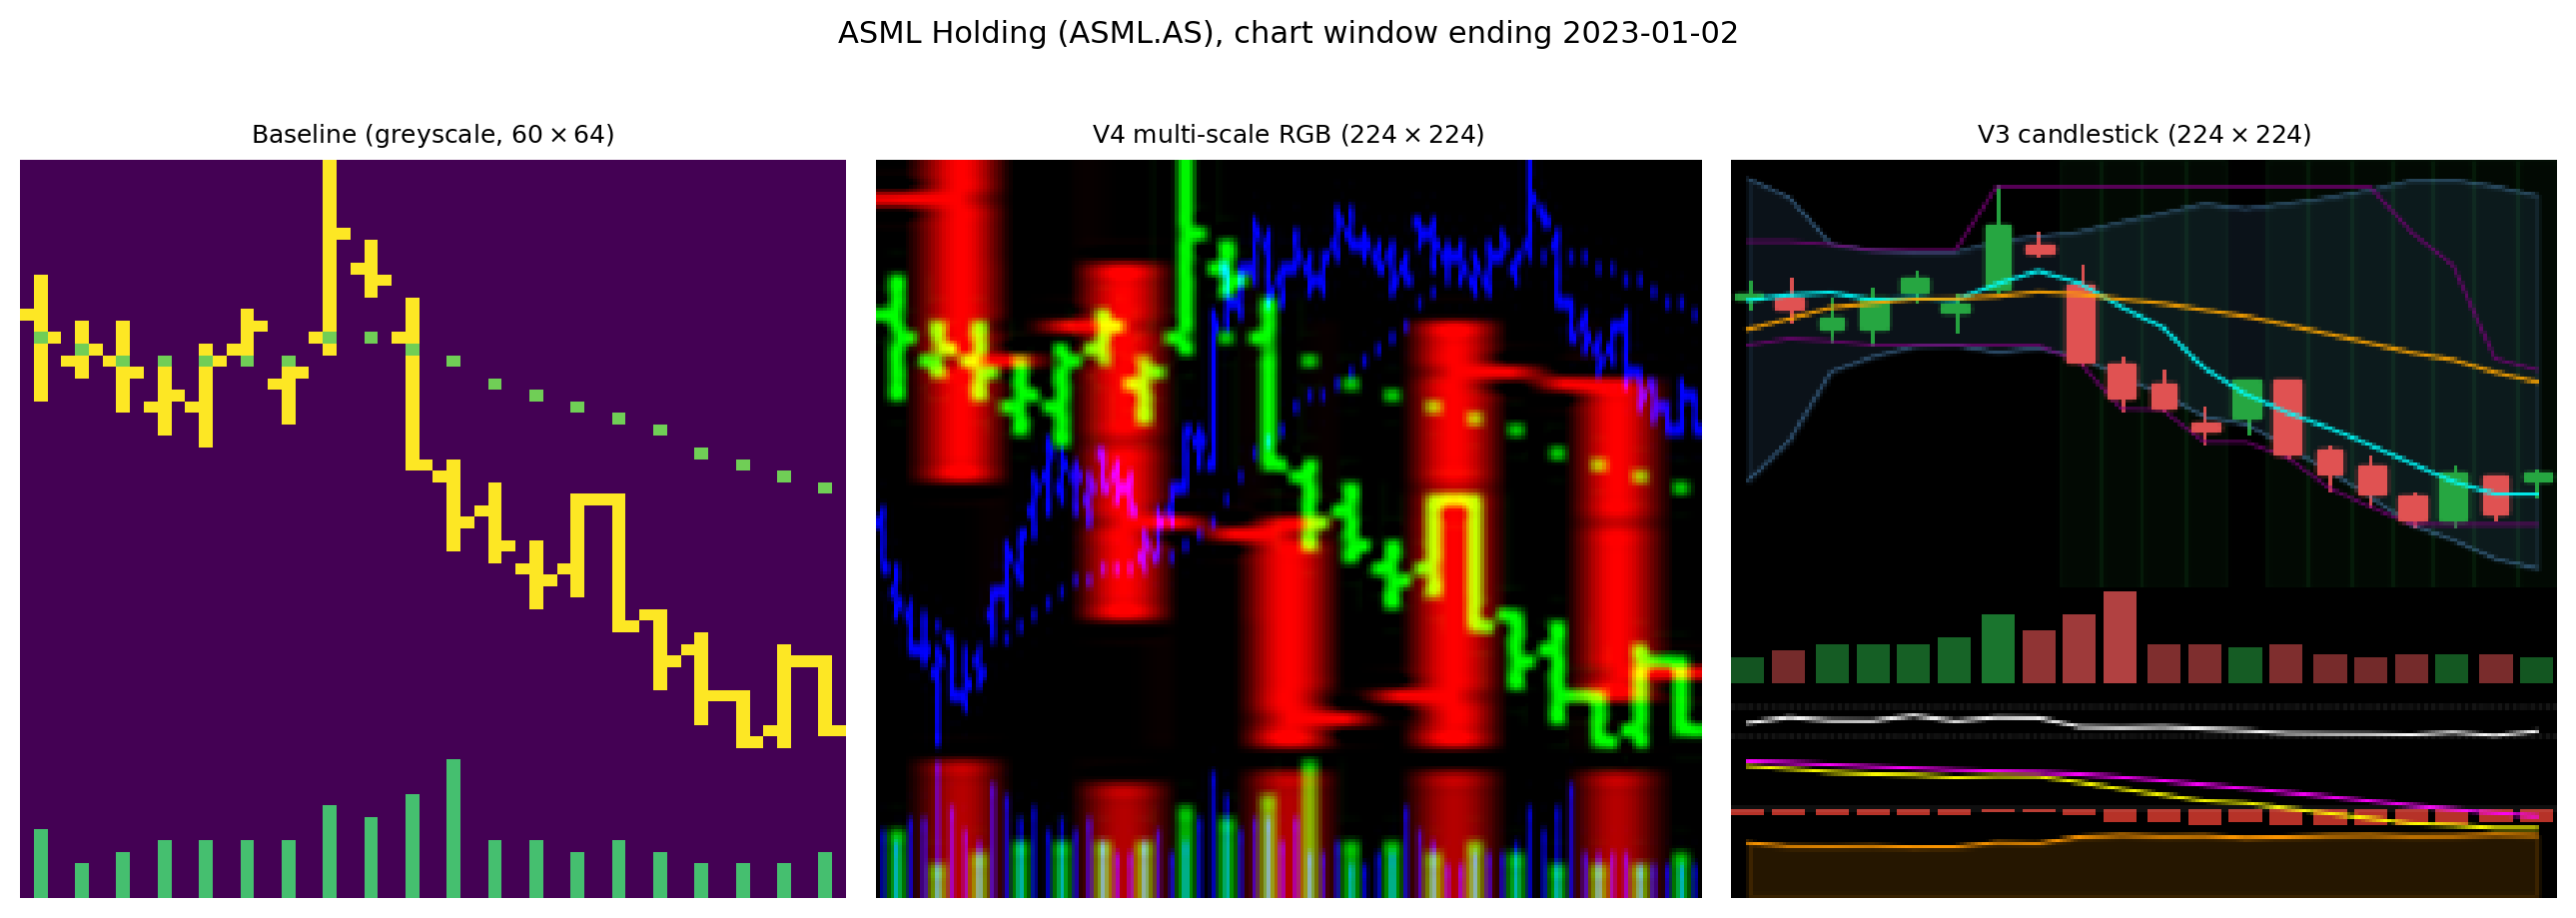
\includegraphics[width=\textwidth]{Graphics/app_image_comparison.png}
\caption{The three chart image formats used in this thesis, shown for ASML Holding on 2 January 2023. Left: Baseline greyscale $60 \times 64$ image following \textcite{Jiang2023}. Centre: V4 multi-scale RGB $224 \times 224$ image with 5-day (Red), 20-day (Green), and 60-day (Blue) OHLC channels. Right: V3 multi-indicator candlestick $224 \times 224$ image with five stacked panels (candlestick, volume, RSI, MACD, ATR).}
\label{fig:app_images}
\end{figure}

\newpage
\section{Extended Portfolio Results}
\label{app:portfolio}

Table~\ref{tab:portfolio_ext} presents portfolio results under both the non-overlapping rebalancing design used in the main analysis and an overlapping version for comparison. The non-overlapping design rebalances every 20 trading days, yielding $N = 65$ independent periods over the five-year test window. The overlapping design forms a new cohort every trading day, with each cohort held for 20 days, and the portfolio return on each day is the average across all active cohorts, producing $N = 1{,}282$ daily observations. Newey-West standard errors use 1 lag for the non-overlapping version and 21 lags for the overlapping version, consistent with the 20-day holding period.

\begin{table}[H]
\centering
\caption{Portfolio Performance: Non-Overlapping vs.\ Overlapping Rebalancing (Test Period 2021--2026)}
\label{tab:portfolio_ext}
\resizebox{\textwidth}{!}{%
\begin{tabular}{llccccc}
\toprule
\textbf{Model} & \textbf{Design} & \textbf{Ann.\ Ret.\ (net)} & \textbf{Sharpe (net)} & \textbf{Sortino (net)} & \textbf{NW $t$} & \textbf{$p$} \\
\midrule
\multirow{2}{*}{Baseline CNN}
  & Non-overlapping ($N=65$)          & $+$3.9\% & 0.32 & 0.54 &  0.77 & 0.446 \\
  & Overlapping ($N=1{,}282$)         & $+$2.3\% & 1.81 & 3.09 &  1.02 & 0.308 \\[4pt]
\multirow{2}{*}{EfficientNet-B2}
  & Non-overlapping ($N=65$)          & $-$0.6\% & $-$0.06 & $-$0.10 & $-$0.15 & 0.884 \\
  & Overlapping ($N=1{,}282$)         & $+$0.5\% &    0.36 &    0.64 &    0.20 & 0.841 \\[4pt]
\multirow{2}{*}{ConvNeXt V2}
  & Non-overlapping ($N=65$)          & $+$3.8\% & 0.36 & 0.62 &  0.87 & 0.389 \\
  & Overlapping ($N=1{,}282$)         & $+$1.8\% & 1.76 & 3.61 &  0.99 & 0.325 \\
\bottomrule
\end{tabular}%
}
\smallskip\par
{\small \textit{Note}: All returns are annualised and net of 10 bps round-trip cost. Sharpe ratios for the overlapping design appear high because overlapping 20-day returns are serially correlated, which compresses the time-series standard deviation. The Newey-West $t$-statistics correct for this and give similar values across both designs. Neither design produces a $t$-statistic above 2.0 for any model.}
\end{table}

The directional conclusion is the same under both approaches: Baseline CNN and ConvNeXt V2 produce positive net returns, EfficientNet-B2 is near zero, and none of the three models achieves conventional statistical significance. The Newey-West $t$-statistics under the overlapping design (1.02, 0.20, 0.99) are close to those from the non-overlapping design (0.77, $-$0.15, 0.87), confirming that the main result does not depend on the choice of rebalancing design.
